% !TeX root = Report.tex
\section{Implemented Algorithms}


\subsection{Tree Aggregation}


\subsection{Clustering}


\subsection{Hierarchical Clustering}

\subsection{HSend}
\begin{itemize}
	\item[] Began with single hop predicates
	\begin{itemize}
		\item used Mesh to gather information from surrounding nodes, due to implementation, we could only send one message as a one time
	\end{itemize}	
	\item[] Started work on Multi-hop local based predicates
	\begin{itemize}
		\item stubborn broadcast to reliably broadcast to one hop neighbours, who would then rebroadcast the message to their neighbours until the hop limit was reached.
		\item We tried using trickle to return the results back to the originating node. However, due to trickles implementation, only one message could be flooded through the network at one time. 
		\item due to collisions, we used ctimers to delay the responses to messages sent back to the originator node.
		\item next step is to re-implement the algorithm, so that nodes send messages directly back along the chain of nodes they recieved the predicated check message from. This way the messages will be more reliably returned to the orignator node. This also allows for multiple messages to be sent this way.
		\item can't really do it via waiting for nodes to respond - difficult to know how long to wait
		\item[] If each node waits (e.g.) 10 seconds, then messages will be lost as they go backwards, as the originating node will have already sent its message back
	\end{itemize}	
\end{itemize}

\subsection{Neighbour Aggregation}

\begin{figure}[ht!]
\centering
\subfigure[Node A requesting neighbour data]{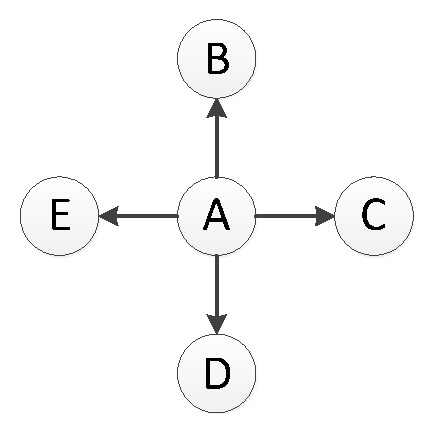
\includegraphics[width=0.25\textwidth]{Diagrams/neighbour-request}}
\subfigure[Node A receiving neighbour data]{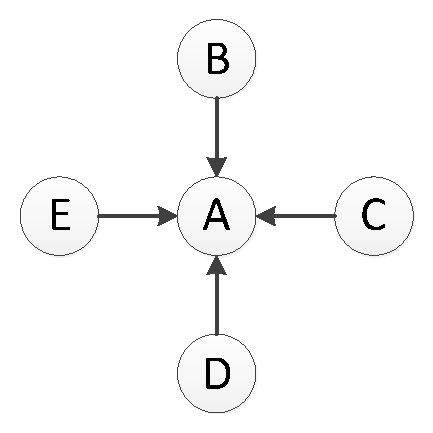
\includegraphics[width=0.25\textwidth]{Diagrams/neighbour-report}}
\end{figure}

\begin{figure}[ht!]
\centering
\subfigure[Example Network]{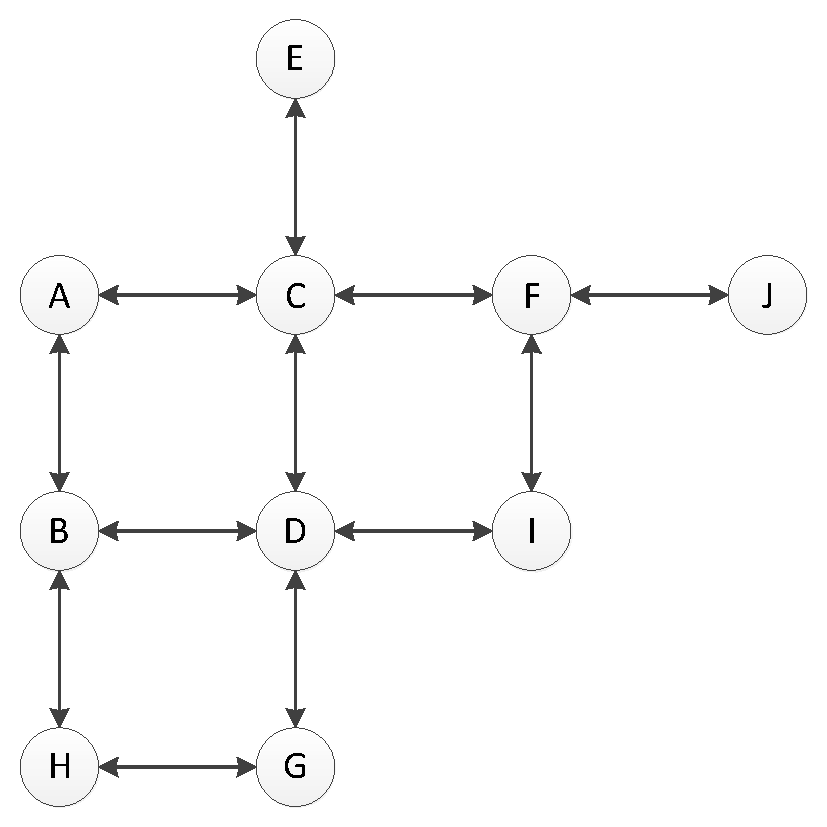
\includegraphics[width=0.75\textwidth]{Diagrams/neighbour-network}}

\subfigure[Logical Tree imposed on network]{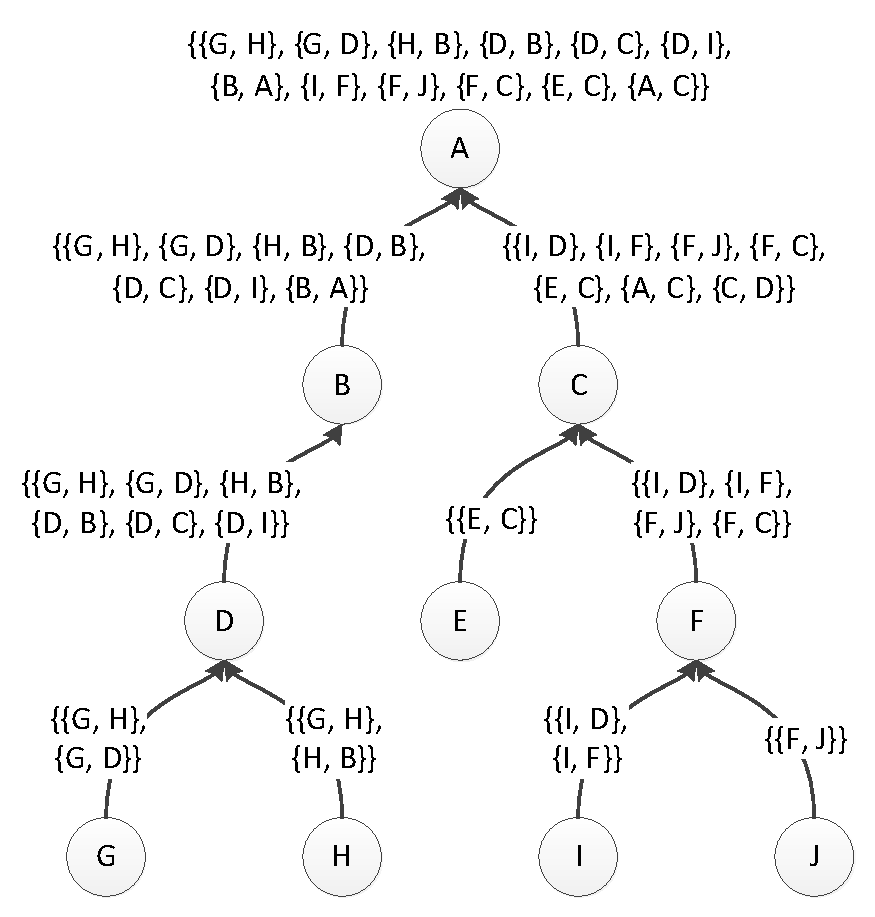
\includegraphics[width=0.75\textwidth]{Diagrams/neighbour-tree-structure}}
\end{figure}



